\chapter*{MAC OS}

\section*{Inicios de Macintosh Operating System}
Más conocido como MAC OS tuvo sus inicios en el año 1984 con el sistema 1.0 que era a blanco y negro, con una pantalla pequeña. inicialmente el sistema operativo mac era instalado en equipos con el diseño de un todo en uno como los de hoy en día con una pantalla de 9 pulgadas y su resolución de 520 x 342. necesitaba 192KB para su instalacion y fue uno de los primeros sistemas operativo en implementar la interfaz del usuario, con la fortuna de haber sido el más exitoso ya que a diferencia de otros sistemas operativos era muy amigable y de facil uso para el usuario.

Algo muy peculiar es que no habia jerarquías de carpetas ya que solo existía una donde se alojaban todos los archivos algo bastante molesto al momento de buscar algún archivo; a diferencia de otros sistemas operativos system 1.0 contaba con un explorador de archivos propio llamado finder que tenia que tenia cuatro menús en la parte superior muy similares a los de hoy en dia.

\section*{Panel de Control}
\begin{figure}
	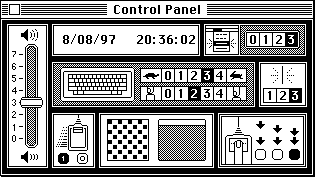
\includegraphics[scale=1]{img/cp09/img0901.png} 
\end{figure}
Definitivamente el panel de control si los va a sorprender, era bastante intuitivo y con funciones muy peculiares, a la izquierda vemos el nivel de volumen, en la parte superior estaba la fecha y hora, el siguiente era para configurar cuantas veces parpadea el menú al momento de seleccionarlo, el menú del centro era un poco confuso ya que es para las repeticiones de las teclas y una velocidad de retraso, el siguiente es la velocidad del cursor al momento estar en un programa de edición de texto, ya en la parte inferior del panel encontramos la velocidad del mouse, el siguiente es para el fondo de pantalla usted dibujaba un patrón a la izquierda y al momento que le daba click en el cuadro de la derecha ya quedaba dibujado en el escritorio y para terminar era ya era para controlar la velocidad del doble click.

Tuve la experiencia de manejar el sistema operativo system software 7.0.1 gracias a un emulador llamado mini vmac y la experiencia como usuario fue bastante agradable ya que el manejo fue muy similar al sistema operativo de hoy dia con la diferencia que al momento de ingresar al menu tenia que tener sostenido el click e ir bajando con el cursor y para seleccionarlo soltar el click, algo muy incomodo, pero en general fue un sistema muy amigable y para las personas de la época creería que era un sistema operativo bastante innovador y llamativo.

\section*{Hoy En Dia Mac OS X Mavericks}
